\chapter{System Design}

%-------------------------------------------------------------------------------------------------------

\section{Requirements Specification}
This section will contain the requirements for this system listed as statements or bullet points, use unambiguous English and avoid technical terms or specifications such as definite language or architecture choices.

\newpage

\subsection{Functional Requirements}

\noindent
\textit{When computing a shortest path the number of vertex accesses should be no more than the total number of vertices.}
\begin{itemize}
\item Input: Map state space containing a goal and a start position.
\item Output: Total number of vertices that are accessed during the computation. \\
\end{itemize}

\noindent
\textit{The total time taken for the autonomous agent to traverse the physical path can be at most 50\% more expensive than a tele-operated agent.}
\begin{itemize}
\item Input: A path of points in Cartesian format. 
\item Output: Time taken in seconds to reach the goal. \\
\end{itemize}

\noindent
\textit{Given an environment containing a start and goal state the path planner must compute a shortest path if one exists.} 
\begin{itemize}
\item Input: Map state space containing a goal and a start position. 
\item Output: A shortest path from the start to the goal or an error if none exists.\\
\end{itemize}

\noindent
\textit{Where there is no traversable path to a goal state the system must immediately abort the planning procedure.} 
\begin{itemize}
\item Input: Map state space containing an unreachable goal. 
\item Output: None. \\
\end{itemize}

\newpage

\subsection{Non-Functional Requirements}

\noindent
\textit{Paths produced by the system should minimise the physical distance to be traversed with the aim of conserving energy resources.} \\

\noindent
\textit{The autonomous agents motion model must be based on a skid steering system that allows for on the spot rotations.} \\

\noindent
\textit{At least one physical courier robot must be capable of carrying out the instructions given to it from the path planning system.} \\

\newpage

%-------------------------------------------------------------------------------------------------------

\section{System Modelling}

\subsection{Overview}
One big diagram of the entire system should feature here, provide the viewer with a complete overview of the system and how everything relates to each other. Explain it in a general way.

\subsection{Interaction Models}
Include various UML based diagrams that show the interactions between the major components in the system the Planner, Algorithm, and Proxy in particular. Keep it high level do not go down into scrupulous detail, focus on communication mechanisms. 

\subsection{Core Class Diagrams}

\noindent
Class diagrams showing relationships between entities such as inheritance, each class diagram should be accompanied with an explanation. Core classes to model include:

\begin{itemize}
\item Robot
\item Proxy
\item Planner
\item Algorithm (abstract)
\item DStarLite (inherits Algorithm)
\item FieldDStar (inherits Algorithm)
\end{itemize} 

\newpage

\subsection{Threaded Architecture}

\noindent
Since threaded programming is notoriously difficult to understand the threading model that the system uses will be covered here in detail, around 1-2 pages. Include a high level diagram and state how each thread interacts with the others. Likely to be around three threads:

\begin{itemize}
\item Main - User interaction
\item Proxy - Robot Communications
\item Planner - Path Planning
\end{itemize} 

\newpage

%-------------------------------------------------------------------------------------------------------

\section{Communications Protocol}\label{sec:protocol}
\noindent
This section briefly discusses the communications protocol that a physical hardware robot must implement in order to be compatible with the planning system. The protocol covered here is an extension of the simple communications mechanism from \cite{JMD14} that was used to drive a tele-operated mapping robot. It is based on plain text strings terminated by new line characters ($\backslash$`n') and was designed with simplicity in mind. All commands are synchronous in behaviour and cannot be completed until the appropriate response has been returned. The complete specification is available in the Appendices under section \ref{Appendix: Communications Protocol Specification}.

\subsection{Message Structure}
\noindent

\subsection{Travelling a Predefined Distance}
\noindent

\subsection{Rotating to a Given Heading}
\noindent

\subsection{Initiating a Scan}
\noindent

\newpage

%-------------------------------------------------------------------------------------------------------

\section{Programming Platforms}

\subsection{Linux Architecture}
\noindent
The Linux kernel is to date driving an increasing number of commercial and research robotic platforms all over the world including Google's Self Car Project \cite{•}, Baxter \cite{•}, Nao \cite{•}, EV3 Lego Mindstorms \cite{•}, and the horde of robots that use ROS \cite{•}. Linux is unique as it is mature, stable, customisable, embeddable, and freely available \cite{•}, making it a suitable candidate for powering the robot revolution. \\

\noindent
\textbf{INSERT PICTURE OF MENTIONED ROBOTS HERE WITH CITATIONS!} \\

\noindent
Considering all of the points previously mentioned Linux was picked as the target programming platform over any other alternatives. Linux's embeddable nature is important to this project as at least one of the physical robots may be equipped with the \textit{Raspberry Pi} \cite{•} a credit card size computer capable of running Linux. The system will be tested on two distributions of Linux, one embedded on the robot(s), the other connected externally:

\begin{itemize}
\item Raspbian ???? (Embedded)
\item Ubuntu Linux 14.10 (External)
\end{itemize} 

\newpage

\subsection{Python3}
Python version 3 (Python3) has been selected as the most appropriate core programming language for the implementation stage for the following reasons:

\begin{itemize}
\item Development Speed - Python is an interpreted bytecode language which is compiled ``on the fly" eliminating lengthy build overheads.
\item Interactive Shell - Python's shell facilitates interactive programming which lends itself to test driven coding.
\item Python and Robotics - already widely used in the robotics field, Sebastian Thurn's Udacity program is done purely using Python \cite{•}.
\end{itemize} 

\noindent
Python's syntax is also extremely lenient when compared to compiled languages such as C where every variable must explicitly declares its type before it can be used, making the equivalent Python code more visually compact. The implementation could have been carried out using C, C++, Java, or C$\sharp$ as the author already has the experience in those languages, however using Python instead presents a unique learning opportunity. 

\subsection{Cython Modules}
\noindent
A major drawback of interpreted languages is the speed of their execution when compared to compiled languages, since Python is implemented using a virtual machine it will nearly always be slower than pure machine code. It is important to take this issue into account at design time as the planning algorithms are computationally complex and as the state space increases Python will become less adapt at handling it compared to a compiled language. \\

\noindent
Fortunately as Python is wrote in C it can also be extend using C. Implementing the planning algorithms as Cython modules shall significantly increase their performance while still enabling the rest of the system to use Python. At the time of writing GCC (GNU C Compiler) version 4.9.1 has been selected for compilation purposes.

\newpage

%-------------------------------------------------------------------------------------------------------

\section{Source Control}
This section covers how the project was managed, the source control system used, frequency off commits, total commits, and any branching.

\subsection{Git}
\noindent
Throughout the projects development all work undertaken including everything from the code base, poster, modelling, and thesis was managed and controlled using the Git source control tool. This decision was taken at design time as it came with a number of distinct advantages such as providing a clear work history and the ability to roll back changes if the need arose. Another important reason for choosing Git over other systems is that it maintains a local copy in addition to the working head in the remote repository \cite{•}. An open repository was set-up and maintained in the cloud at the GitHub \href{https://www.github.com/swordmaster2k/botnav}{BotNav}.

%-------------------------------------------------------------------------------------------------------

\section{Hardware Agent Specification}
\noindent
As the path planning system implemented on the Linux host is designed to be independent from the hardware specifics of the robot it is necessary that all robots communicate with the planner in a predefined way. We have all ready discussed this mechanism under \ref{sec:protocol} from the software side now it is time to specify a generic robot that implements the interface. \\

\noindent
In order to be compatible with the planner a robot must have software/hardware:

\begin{itemize}
\item Odometers - capable of establishing an $(x, y)$ position in meters and $\theta$ in radians.
\item Communications - a channel for processing text based data to and from the planner.
\item External Sensors - at least one proximity sensor for detecting obstacles in the environment.
\end{itemize}

\newpage

\noindent
How accurate this hardware needs to be is completely dependent on the application, the planning system can only assume that any data it receives is valid. Any hardware inaccuracies i.e. drift must be dealt with at a lower level, the purpose of this approach is to decouple the planner from a robot's implementation details. This enables the planning system to be tested across a wide variety of platforms without having to account for each individual hardware configuration (Figure \ref{Figure: Hardware Agent Specification.}). It is perfectly possible that the planner and robot hardware control be implemented on the same physical system rather than externally this could be done via IP using the \textit{localhost} address.

\begin{figure}[htbp]

\center 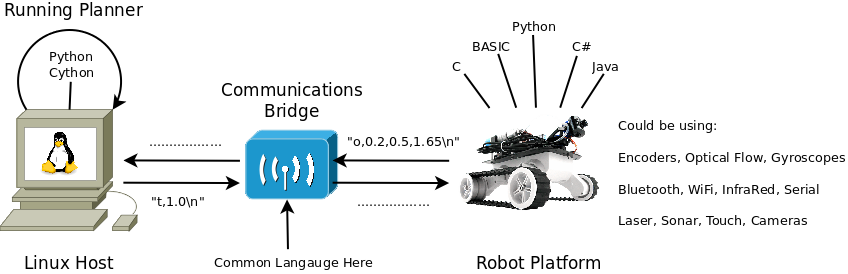
\includegraphics[width=400pt]{illustrations/hardware_agent_specification}\\
\caption{The planner on the Linux host and robot platform communicate via a common communications bridge that they both understand regardless of implementation details.} 
\label{Figure: Hardware Agent Specification.}

\end{figure}

\noindent
Talk about a specific case for a robot probably the microbot or something here...


\subsection{Motion Model}
\noindent
The planner will impose some restrictions on the motion model that a robot must use to be compatible with the paths it produces. It will be assumed that the robot can perform on the spot rotations, this is necessary as all of the path planning algorithms \textit{may} produce paths that require this kind of motion. In wheeled and tracked vehicles this is typically referred to as \textit{skid steering} \cite{building robot drive trains}, on the spot rotations are achieved by running the drive systems on either side in opposite directions, a tank is good example of this. Legged robots are also capable of performing such turns, however the heading changes can be too extreme for rack-and-pinion based agents i.e. cars and trucks. 

\newpage

%-------------------------------------------------------------------------------------------------------
